\documentclass[a4paper,12pt,twoside]{scrreprt}
% Autor der Vorlage: Klaus Rheinberger, FH Vorarlberg
% 2017-02-20

%% Hilfe: z.B.
% empfohlener Einstieg: http://latex.tugraz.at/  
% https://de.wikibooks.org/wiki/LaTeX-Kompendium:_Schnellkurs:_Erste_Schritte
% https://de.wikibooks.org/wiki/LaTeX-Kompendium:_Schnellkurs
% https://de.wikibooks.org/wiki/LaTeX-Kompendium

%% Pakete:
% Der Befehl \usepackage[latin9]{inputenc} ermöglicht die direkte Angabe von Umlauten. Übrigens lässt sich so auch das Euro-Zeichen direkt eingeben. Auf Betriebssystemen, wie zum Beispiel allen neueren Linux-Distributionen, verwendet man statt \usepackage[latin9]{inputenc} besser \usepackage[utf8]{inputenc}, auf Applesystemen verwendet man \usepackage[macce]{inputenc} (oder das für ältere Modelle gültige \usepackage[applemac]{inputenc}).
\usepackage[utf8]{inputenc}
\usepackage[T1]{fontenc}    % Silbentrennung bei Sonderzeichen
\usepackage{graphicx}       % Bilder einbinden
\usepackage{lscape}         % Querformat
\usepackage[ngerman]{babel} % Deutsche Sprachanpassungen
\usepackage{footnote}       % footer citations
\usepackage{csquotes}       % When using babel or polyglossia with biblatex, loading csquotes is recommended to ensure that quoted texts are typeset according to the rules of your main language.
\usepackage{acronym}  % für optionales Abkürzungsverzeichnis
\usepackage[linktocpage=true]{hyperref} % Links z. B. \href{https://www.wikibooks.org}{Wikibooks home}
\usepackage{caption} % Abbildungslegenden
\usepackage{booktabs} % schönere horizontale Trennlinien für Tabellen 
\captionsetup{format=hang, justification=raggedright}
\usepackage[style=verbose,backend=bibtex]{biblatex}   % Literaturverweise
% biblatex comes with a variety of built-in bibliography/citation style families (numeric, alphabetic, authoryear, authortitle, verbose), and there's a growing number of custom styles:
% https://de.sharelatex.com/learn/Biblatex_citation_styles
% https://de.sharelatex.com/learn/Biblatex_bibliography_styles
\addbibresource{bibliography.bib}    % Zotero-Beispiele.bib ist die verwendete Bibtex-Datei 
% Anstatt die Bibtex-Datei selber zu erstellen, kann sie z. B. aus einer Zotero-Sammlung zu BibTeX exportiert werden.

% float package
\usepackage{float}

% fußnotennummerierung nicht neu beginnen in jedem kapitel
\usepackage{chngcntr}
\counterwithout*{footnote}{chapter}

% enumitem for enumarations
\usepackage{enumitem}
\setlist[1]{itemsep=0pt,parsep=0px}

% use for side-by-side figures
\usepackage{subfigure}

%% Einstellungen:
\setcounter{secnumdepth}{4}
\setcounter{tocdepth}{4}   % Tiefe der Gliederung im In haltsverzeichnis


%% ERSETZEN VON ECKIGEN KLAMMERN:
% Ersetzen Sie den Text in den eckigen Klammern!

\begin{document}

% evtl. Sperrvermerkseite
\thispagestyle{empty}
[Achtung: Verwenden Sie einen Sperrvermerk nur in sehr gut begründeten Fällen!] 

\section*{[evtl. Sperrvermerk]}   % evtl. ersetzen durch \section*{Sperrvermerk}
Auf Wunsch der Firma [FIRMA] ist die vorliegende Arbeit bis zum [DATUM] für die öffentliche Nutzung zu sperren. 

Veröffentlichung, Vervielfältigung und Einsichtnahme sind ohne ausdrückliche Genehmigung der oben genannten Firma und der/dem Verfasser/in nicht gestattet. Der Titel der Arbeit sowie das Kurzreferat/Abstract dürfen jedoch veröffentlicht werden.

\vspace{3cm}

\noindent Dornbirn, \hfill Unterschrift der Verfasserin/des Verfassers

\vspace{2cm}

\hfill Firmenstempel\hspace{2cm}


% Titelblatt:
% \newpage\mbox{}\newpage

% force output to a right page
\cleardoublepage{}
\thispagestyle{empty}
\begin{titlepage}
  \begin{flushright}
  
\includegraphics[width=0.4\linewidth]{Logo-A3}
  \end{flushright}
  \begin{flushleft}
  \section*{Qualitätsmanagement in Scrum-Teams}
  \subsection*{Untertitel}
  \vspace{1.5cm}
  
  Masterarbeit\\
  zur Erlangung des akademischen Grades
  \vspace{0.5cm}
  
  \textbf{Master of Science (MSc)}

  \vspace{2cm}
  Fachhochschule Vorarlberg\newline
  Informatik

  \vspace{1cm}
  
  Betreut von\newline
  Prof.\ Dr.\ Michael Felderer
  
  \vspace{2cm}
  
  Vorgelegt von\newline
  Daniel Grießer\newline
  Dornbirn, Juli 2018
  \end{flushleft}
\end{titlepage}

% Kurzreferat:
\newpage
\section*{Kurzreferat}

\subsection*{[Deutscher Titel Ihrer Arbeit]}

[Text des Kurzreferats]


% Abstract:
\newpage
\section*{Abstract}
\subsection*{[English Title of your thesis]}

[text of the abstract]


% Inhaltsverzeichnis:
\cleardoublepage\tableofcontents

\clearpage
\phantomsection\addcontentsline{toc}{chapter}{Abbildungsverzeichnis}
\listoffigures

\clearpage
\phantomsection\addcontentsline{toc}{chapter}{Tabellenverzeichnis}
\listoftables

% Abkürzungsverzeichnis:
\clearpage
\phantomsection\addcontentsline{toc}{chapter}{Abkürzungsverzeichnis}
\chapter*{Abkürzungsverzeichnis}
\begin{acronym}
    \acro{APM}{Application-Performance-Monitoring}
    \acro{BI}{Business-Intelligence}
    \acro{CD}{Continuous Delivery}
    \acro{CI}{Continuous Integration}
    \acro{CLOC}{Changed Lines of Code}
    \acro{DoD}{Definition of Done}
    \acro{EAT}{Executive Action Team}
    \acro{EMS}{Executive Meta Scrum}
    \acro{FCM}{Factor Criteria Metrics}
    \acro{GQM}{Goal Question Metric}
    \acro{IEEE}{Institute of Electrical and Electronics Engineers}
    \acro{LeSS}{Large Scale Scrum}
    \acro{LOC}{Lines of Code}
    \acro{MTTF}{Mean Time to Failure}
    \acro{MTTR}{Mean Time to Release}
    \acro{NASA}{National Aeronautics and Space Administration}
    \acro{NoSQL}{Not-only-SQL}
    \acro{PBR}{Product Backlog Refinement}
    \acro{PTS}{Project Tracking System}
    \acroplural{PTS}[PTS]{Project Tracking Systems}
    \acro{QS}{Qualitätssicherung}
    \acro{SoS}{Scrum of Scrums}
    \acro{VCS}{Version Control System}
    \acroplural{VCS}[VCS]{Version Control Systems}
\end{acronym}


%% Die Kapitelstruktur ist mit der Betreuungsperson abzustimmen!
\chapter{Einleitung}

Dieses Kapitel gibt eine kurze Übersicht über den Aufbau und die Motivation hinter dieser Arbeit.

\section{Zielsetzung}

Agile Prozesse, insbesondere Scrum, basieren auf empirischen, also durch fortlaufende Beobachtung erhobenen und auswertenden, Daten (siehe Abschnitt~\ref{section:scrum}).
Das bedeutet, dass sich der Prozess durch Reflexion verbessert und auch Veränderung zulässt.
Um diese Reflexion zu vereinfachen, ist es hilfreich, gewisse Kennzahlen des Prozesses und des Produktes grafisch darzustellen.
Im Speziellen Metriken können eine gute qualitative Auskunft über den aktuellen Status geben.
Ziel dieser Arbeit soll es sein, Metriken zu ermitteln, die Qualitätsprobleme im Entwicklungsprozess oder im Softwareprodukt quantitativ abbilden können.
Weiters sollen diese Metriken gesammelt und grafisch dargestellt werden.
Sie können aus Daten generiert werden, die bei der tagtäglichen Arbeit in den jeweiligen Systemen erzeugt werden.
Solche Systeme reichen von \acfp{VCS}, über \acfp{PTS} und \acf{CI} / \acf{CD}, bis hin zu \acf{APM}.
Diese Daten können meist über Schnittstellen abgefragt und anschließend aggregiert abgelegt werden.
Umgesetzt wird das Ganze in einem relativ jungen, aber im Scrum Prozess bereits weit fortgeschrittenen Scrum-Team.

\clearpage
\section{Aufbau der Arbeit}

Nach der Einleitung gibt das Kapitel ``Stand der Technik'' einen Einblick in die unterschiedlichen Themen und die theoretischen Hintergründe dieser Arbeit.
Zuerst werden die Grundsäulen der agilen Softwareentwicklung, das agile Manifest und die agilen Prinzipien, genauer erklärt.
Darauf folgend wird auf Scrum eingegangen und zusätzlich Ansätze für Scrum in mehreren Teams erklärt.
Anschließend wird zu Qualität übergegangen, im Speziellen Software- und Prozessqualität.
Basierend auf den beiden vorherigen Themen, wird dann genauer auf Metriken eingegangen, was auch der Hauptteil dieses Kapitels darstellt.
Im ersten Teil werden Metriken aus den unterschiedlichsten Systemen vorgestellt und wie eigene Metriken erstellt werden können.
Danach folgen Hinweise zur Veröffentlichung von Metriken und der Messung von Agilen Prinzipien.
Am Schluss folgen noch ein Überblick über Qualitätsmodelle und das \ac{GQM}-Modell, sowie das \ac{FCM}-Modell im Detail.
\\
Im Kapitel ``Vorgehensweise'' wird beschrieben, wie bei der Bestimmung der relevanten Metriken für das Team, bei der Erstellung der Software und bei der Evaluierung der Ergebnisse vorgegangen wird.
\\
Das Kapitel ``Umsetzung'' zeigt dann, wie der Titel schon sagt, die Umsetzung der Lösung.
Anfangs werden die Gegebenheiten erläutert, in der die Lösung eingesetzt wird.
Dann wird mit der Identifizierung der Metriken gestartet und diese anschließend in der entwickelten Software gesammelt.
Zuletzt wird noch genauer auf die Darstellung eingegangen.
\\
Es folgt das Kapitel ``Evaluierung'', in dem die Ergebnisse qualitativ in Form von Interviews und quantitativ in Form der Metriken evaluiert werden.
In den Kapiteln ``Schlussfolgerungen'' und ``Zusammenfassung'' werden die Ergebnisse nochmal reflektiert, zusammengefasst und ein Ausblick für mögliche weitere Arbeiten gegeben.

\chapter{Situationsanalyse}

\section{Agile Softwareentwicklung}

Diese Arbeit dreht sich um agile Teams, deshalb ist es essentiell, zu verstehen, was der Gedanke hinter dem agilen Entwicklungsansatz ist.
Seinen Ursprung hat das Ganze, als sich 2001 ein paar schlaue Köpfe zusammengeschlossen haben und das sogenannte agile Manifest, sowie die agilen Prinzipien aufgestellt haben.
Ziel war es, eine Alternative zu den bisherigen, schwergewichtigen und von Dokumentation getriebenen Softwareentwicklungs-Methodologien zu finden.

\subsection{Agiles Manifest}

Das agile Manifest ist er Grundbaustein aller agilen Vorgehensmodelle:

\begin{quote}Wir erschließen bessere Wege, Software zu entwickeln,
indem wir es selbst tun und anderen dabei helfen.
Durch diese Tätigkeit haben wir diese Werte zu schätzen gelernt: \newline
\begin{center}
Individuen und Interaktionen mehr als Prozesse und Werkzeuge \newline
Funktionierende Software mehr als umfassende Dokumentation \newline
Zusammenarbeit mit dem Kunden mehr als Vertragsverhandlungen \newline
Reagieren auf Veränderung mehr als das Befolgen eines Plans \newline
\end{center}
Das heißt, obwohl wir die Werte auf der rechten Seite wichtig finden,
schätzen wir die Werte auf der linken Seite höher ein.\end{quote}\cite{agile_manifest}

\subsection{Agile Prinzipien}

Die agile Softwareentwicklung folgt diesen zwölf Prinzipien:

\begin{quote}Unsere höchste Priorität ist es, den Kunden durch frühe und kontinuierliche Auslieferung wertvoller Software zufrieden zu stellen.

Heisse Anforderungsänderungen selbst spät in der Entwicklung willkommen. Agile Prozesse nutzen Veränderungen zum Wettbewerbsvorteil des Kunden.

Liefere funktionierende Software regelmäßig innerhalb weniger Wochen oder Monate und bevorzuge dabei die kürzere Zeitspanne.

Fachexperten und Entwickler müssen während des Projektes täglich zusammenarbeiten.

Errichte Projekte rund um motivierte Individuen. Gib ihnen das Umfeld und die Unterstützung, die sie benötigen und vertraue darauf, dass sie die Aufgabe erledigen.

Die effizienteste und effektivste Methode, Informationen an und innerhalb eines Entwicklungsteams zu übermitteln, ist im Gespräch von Angesicht zu Angesicht.

Funktionierende Software ist das wichtigste Fortschrittsmaß.

Agile Prozesse fördern nachhaltige Entwicklung. Die Auftraggeber, Entwickler und Benutzer sollten ein gleichmäßiges Tempo auf unbegrenzte Zeit halten können.

Ständiges Augenmerk auf technische Exzellenz und gutes Design fördert Agilität.

Einfachheit -\phantom{}- die Kunst, die Menge nicht getaner Arbeit zu maximieren -\phantom{}- ist essenziell.

Die besten Architekturen, Anforderungen und Entwürfe entstehen durch selbstorganisierte Teams.

In regelmäßigen Abständen reflektiert das Team, wie es effektiver werden kann und passt sein Verhalten entsprechend an.\end{quote}\cite{agile_principles}

\section{Scrum (Quellenangabe!)}

Das Scrum Framework ist eine solche agile Softwareentwicklungs-Methodologie. 
Scrum basiert auf Empirismus, also der Theorie, dass Wissen aus Erfahrung erlangt wird und Entscheidungen auf Basis dieses Wissens getroffen werden. 
Die drei Grundsäulen einer solchen empirischen Prozesskontrolle sind:

\begin{description}
  \item[Transparenz] \hfill \\ Signifikante Aspekte des Prozesses müssen für alle sichtbar sein.
  \item[Inspektion] \hfill \\ Artefakte müssen regelmäßig inspiziert werden, aber dieser Vorgang darf der Arbeit selbst nicht im Weg stehen.
  \item[Adaption] \hfill \\ Weicht ein oder mehrere Aspekte eines Prozesses von seinen akzeptablen Limits ab, muss dieser so früh wie möglich angepasst werden.
\end{description}

Das Scrum Framework (Abbildung~\ref{fig:scrum_framework}) besteht aus drei Rollen, fünf Ereignissen und drei Artefakten.

\begin{itemize}
  \item \textbf{Rollen}
  \begin{itemize}
    \item \textbf{Development Team}: Selbstorganisiertes Team, das am Produkt arbeitet.
    \item \textbf{Scrum Mater}: Verantwortlich dafür, sicherzustellen, dass Scrum verstanden und gelebt wird.
    \item \textbf{Product Owner}: Verantwortlich den Wert des Produktes und die Arbeit des Development Teams zu maximieren.
  \end{itemize}
  \item \textbf{Ereignisse}
  \begin{itemize}
    \item \textbf{Sprint}: Ist das Herz von Scrum: eine Timebox von 2 bis 4 Wochen, in dem ein fertiges, verwendbares und potentiell releasebares Produkt-Inkrement entwickelt wird.
    \item \textbf{Sprint Planning}: Planung eines Sprints. Hier commited sich das Scrum Team, eine gewisse Anzahl an Aufgaben im kommenden Sprint abzuarbeiten.
    \item \textbf{Daily Scrum}: Tägliches, zeitlich begrenztes Meeting, bei dem von jedem Teammitglied folgende drei Fragen beantwortet werden:
    \begin{enumerate}
      \item Was habe ich gemacht?
      \item Was werde ich machen?
      \item Was behindert mich bei meiner Arbeit?
    \end{enumerate}
    \item \textbf{Sprint Review}: Abschluss eines Sprints. Hier präsentiert das Team dem Product Owner die Ergebnisse des letzten Sprints.
    \item \textbf{Sprint Retrospective}: Das Team reflektiert den Sprint-Ablauf und ergreift Maßnahmen, um den Prozess weiter zu verbessern.
  \end{itemize}
  \item \textbf{Artefakte}
  \begin{itemize}
    \item \textbf{Product Backlog}: Ist eine Sammlung von möglichen Aufgaben für das Team am Produkt. Sollte einen Ausblick auf die zukünftige Entwicklung des Produktes geben. Oben im Product Backlog befinden sich die bereits fein geplanten Aufgaben, weiter unten die groben.
    \item \textbf{Sprint Backlog}: Entspricht den Aufgaben, die vom Team in den Sprint genommen und dem Product Owner zugesagt wurden.
    \item \textbf{Increment}: Entsteht am Ende eines jeden Sprints und ist eine lauffähige Version des Produkts, die releasefähig ist.
  \end{itemize}
\end{itemize}

\begin{savenotes}
  \begin{figure}[H] 
    \centering
       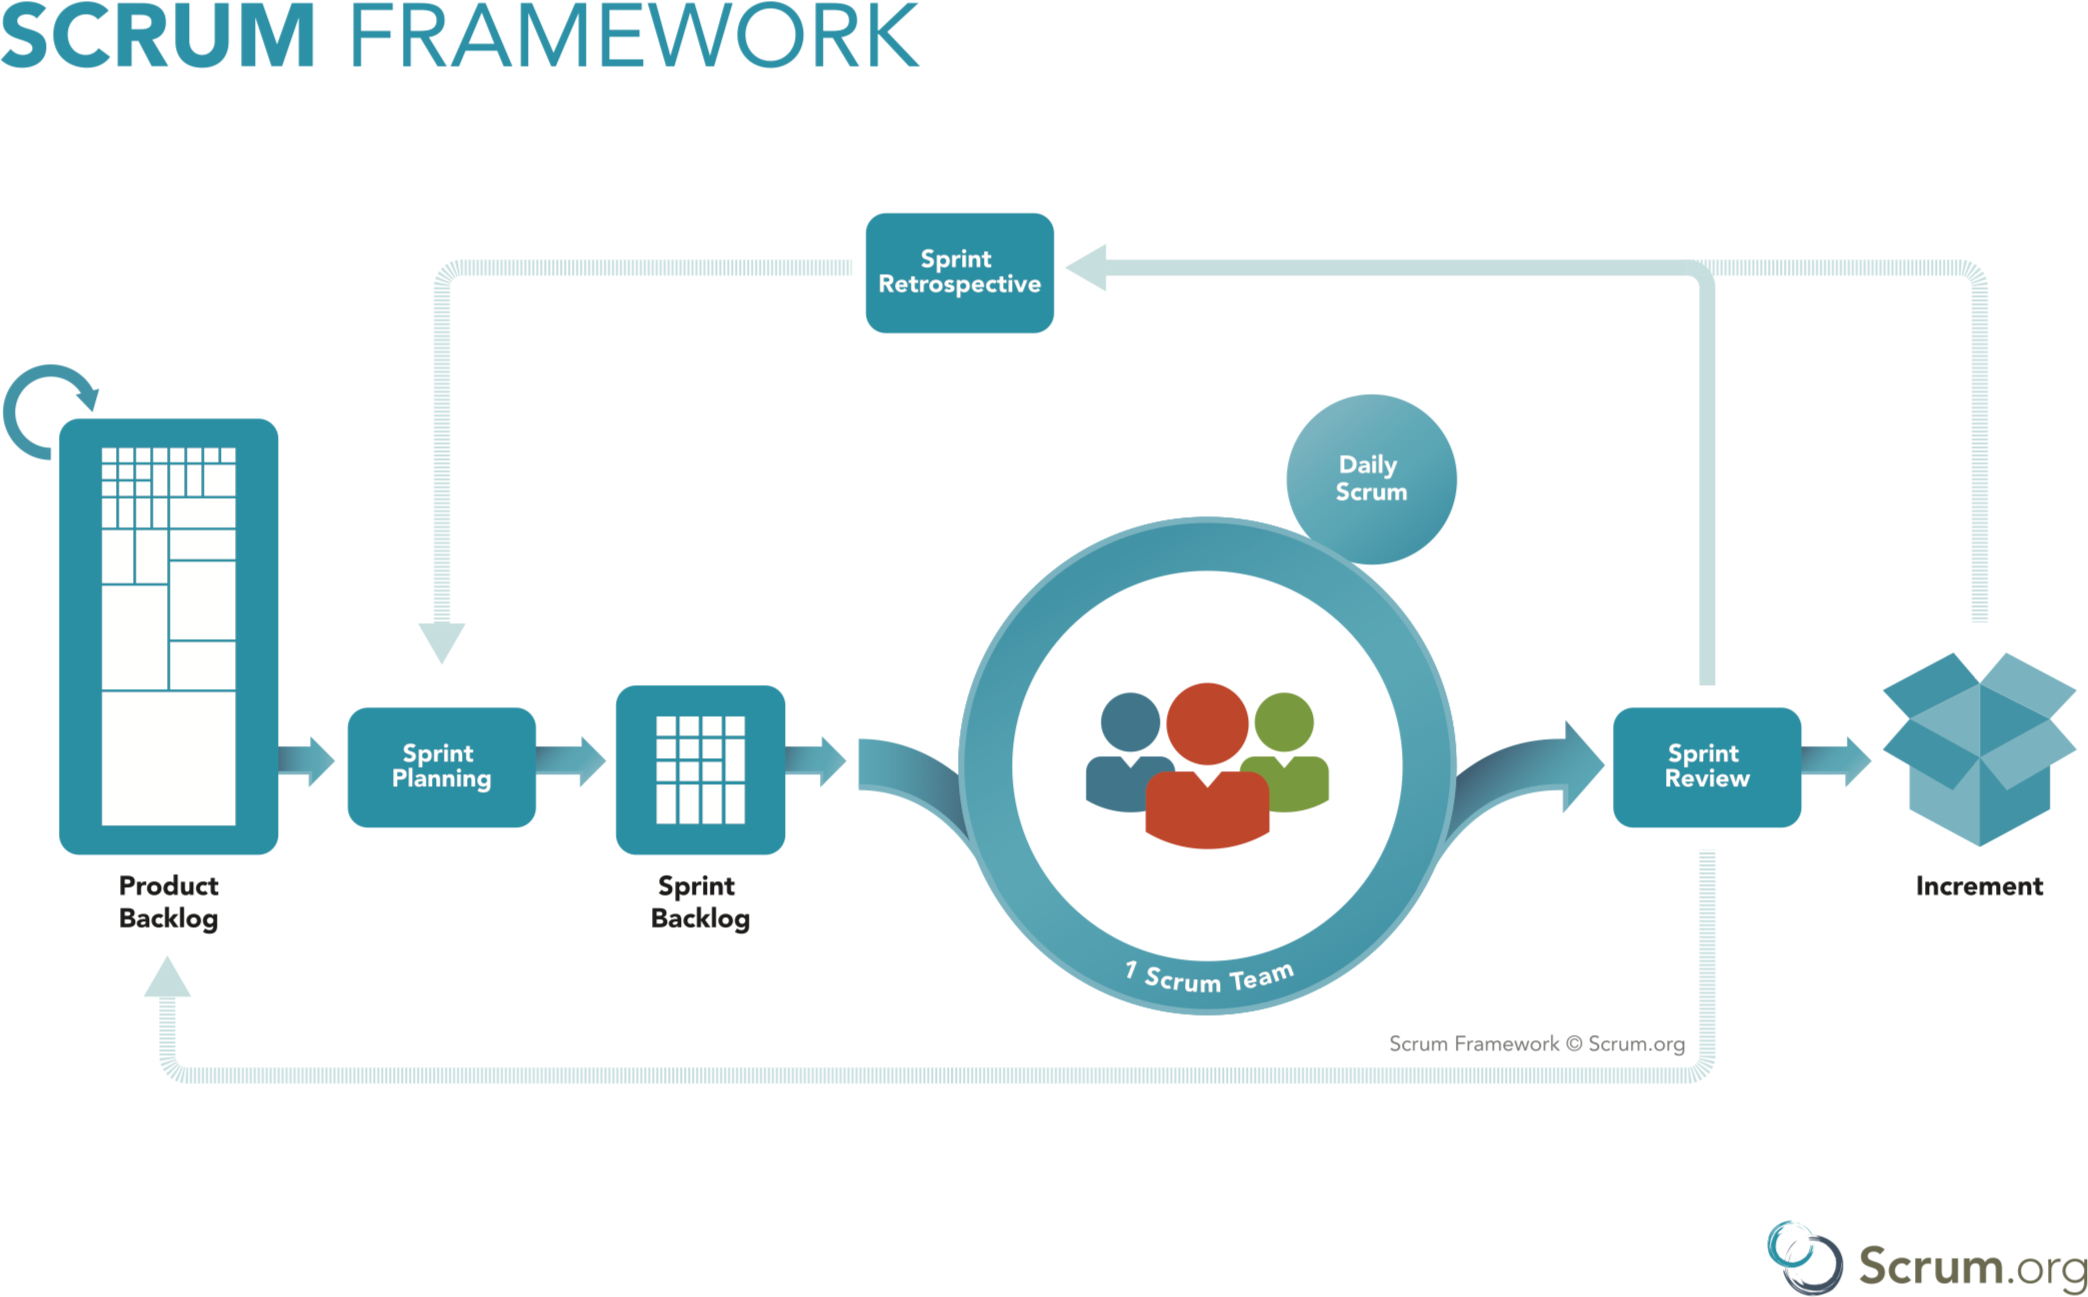
\includegraphics[width=0.9\textwidth]{img/scrum-framework.png}
    \caption[Scrum Framework]{Scrum Framework~\footcite{scrum_framework}}\label{fig:scrum_framework}
  \end{figure}
\end{savenotes}

\subsection[Scrum in mehreren Teams]{Scrum in mehreren Teams~\footcite[vgl.][S.172ff]{scrum_kurz_gut_2013}}

Scrum beschreibt eine agile Vorgehensweise für ein Team (ein Team entwickelt ein Produkt).
In der Realität existieren aber oft mehrere Teams und/oder mehrere Produkte. 
Dahingehend muss die Organisation der unterschiedlichen Scrum Teams individuell angepasst werden.
Für die Trennung der Teams gibt es unterschiedliche Ansätze:
\begin{description}
  \item[Trennung nach Organisationseinheiten] \hfill \\ Die Teams werden entlang der Abteilungsstruktur einer Organisation getrennt. Aus Scrum-Sicht macht das nicht immer Sinn, da bei der Umsetzung eines Features Abhängigkeiten zu anderen Teams bestehen (keine cross-funktionalen Teams).
  \item[Trennung nach Komponenten (Komponenten-Teams)] \hfill \\ Die technischen Komponenten werden den Teams zugeteilt, was ebenfalls zu Abhängigkeiten zu anderen Teams führt und eine gute Abstimmung zwischen den Teams voraussetzt.
  \item[Trennung nach fachlichen Themen (Feature-Teams)] \hfill \\ Jedes Team entwickelt, unabhängig von den anderen Teams, eine fachliche Komponente. Diese Variante erfüllt die Forderung des Scrum Frameworks nach cross-funktionalen Teams, weshalb bei dieser Form die Abstimmung zwischen den Teams am geringsten ist.
\end{description}

\begin{savenotes}
  \begin{figure}[H]
    \centering
    \subfigure[Feature-Teams]{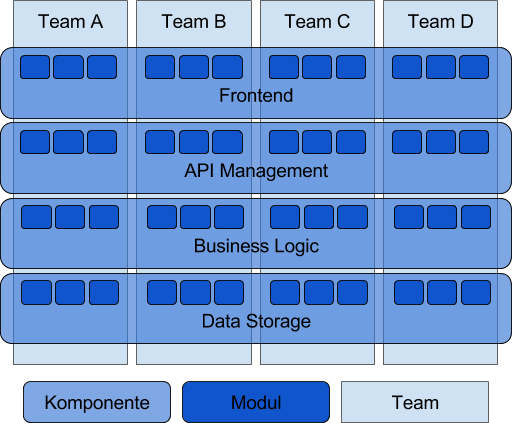
\includegraphics[width=0.40\textwidth]{img/feature-teams.png}} 
    \subfigure[Komponenten-Teams]{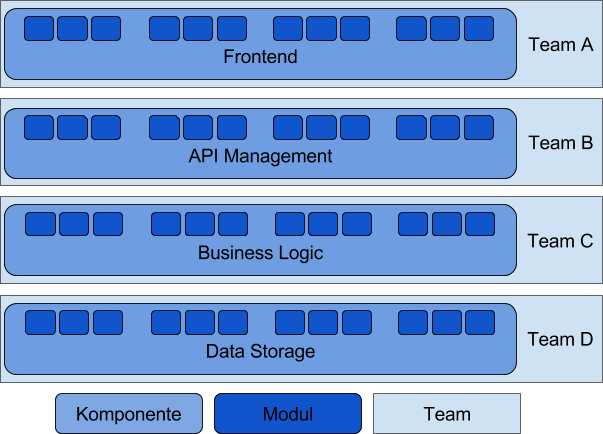
\includegraphics[width=0.48\textwidth]{img/component-teams.png}} 
  \caption{Scrum Teams}\label{fig:Scrum Teams}
  \end{figure}
\end{savenotes}

In allen Varianten existieren aber pro Team unterschiedliche Software-Module und (agile) Prozesse, die unabhängig voneinander die Team-Qualität als gesamtes bestimmen.

\clearpage
\section[Software-Qualität]{Software-Qualität~\footcite[vgl.][Kapitel 1.2]{hoffmann_software_qualitat_2013}}

Eine mögliche Definition von Software-Qualität findet sich in der DIN-ISO-Norm 9126:

\begin{quote}
  ``Software-Qualität ist die Gesamtheit der Merkmale und Merkmalswerte eines Software-Produkts, die sich auf dessen Eignung beziehen, festgelegte Erfordernisse zu erfüllen.''
\end{quote}

Wie aus dieser Definition schon erkennbar ist, gibt es viele unterschiedliche Kriterien, um die Qualität von Software zu bewerten.
Einige wesentliche Merkmale, um die Qualität von Software bewerten zu können, lassen sich in kunden- und herstellerorientierte Merkmale unterteilen:

\begin{description}
  \item[Kundenorientierte Merkmale] \hfill \\ Nach außen hin sichtbare Merkmale, die sich auf den kurzfristigen Erfolg der Software auswirken, da sie die Kaufentscheidung möglicher Kunden beeinflussen.
  \begin{description}
    \item[Funktionalität (Functionality, Capability)] \hfill \\ Beschreibt die Umsetzung der funktionalen Anforderungen. Fehler sind hier häufig Implementierungsfehler (sogenannte Bugs), welche durch Qualitätssicherung bereits in der Entwicklung entdeckt oder vermieden werden können. 
    \item[Laufzeit (Performance)] \hfill \\ Beschreibt die Umsetzung der Laufzeitanforderungen. Besonderes Augenmerk muss in Echtzeitsystemen auf dieses Merkmal gelegt werden.
    \item[Zuverlässigkeit (Reliability)] \hfill \\ Eine hohe Zuverlässigkeit ist in kritischen Bereichen, wie z.B. Medizintechnik oder Luftfahrt, unabdingbar. Erreicht werden kann diese aber nur durch die Optimierung einer Reihe anderer Kriterien.
    \item[Benutzbarkeit (Usability)] \hfill \\ Betrifft alle Eigenschaften eines Systems, die mit der Benutzer-Interaktion in Berührung kommen.
  \end{description}
  \item[Herstellerorientierte Merkmale] \hfill \\ Sind die inneren Merkmale, die sich auf den langfristigen Erfolg der Software auswirken und somit als Investition in die Zukunft gesehen werden sollten.
  \begin{description}
    \item[Wartbarkeit (Maintainability)] \hfill \\ Die Fähigkeit auch nach der Inbetriebnahme noch Änderungen an der Software vorzunehmen. Wird oft vernachlässigt, ist aber essentiell für langlebige Software und ein großer Vorteil gegenüber der Konkurrenz.
    \item[Transparenz (Transparency)] \hfill \\ Beschreibt, wie die nach außen hin sichtbare Funktionalität intern umgesetzt wurde. Gerade bei alternder Software, kann es zu einer Unordnung kommen, welche auch Software-Entropie (Grad der Unordnung) genannt wird.
    \item[Übertragbarkeit] \hfill \\ Wird auch Portierbarkeit genannt und beschreibt die Eigenschaft einer Software, in andere Umgebungen übertragen werden zu können (z.B. 32-Bit zu 64-Bit oder Desktop zu Mobile).
    \item[Testbarkeit (Testability)] \hfill \\ Testen stellt eine große Herausforderung dar, da oft auf interne Zustände zugegriffen werden muss oder die Komplexität die möglichen Eingangskombinationen vervielfacht. Aber gerade durch Tests können Fehler frühzeitig entdeckt und behoben werden.
  \end{description}
\end{description}

Je nach Anwendungsgebiet und den Anforderungen der Software haben die Merkmale unterschiedliche Relevanz und einige können sich auch gegenseitig beeinflussen, wie aus der Korrelationsmatrix in Abbildung~\ref{fig:scrum_framework} ersichtlich.
Dabei sind die positiv korrelierenden Merkmale mit ``+'' und die negativ korrelierenden mit ``-'' gekennzeichnet.

\begin{savenotes}
  \begin{figure}[H] 
    \centering
       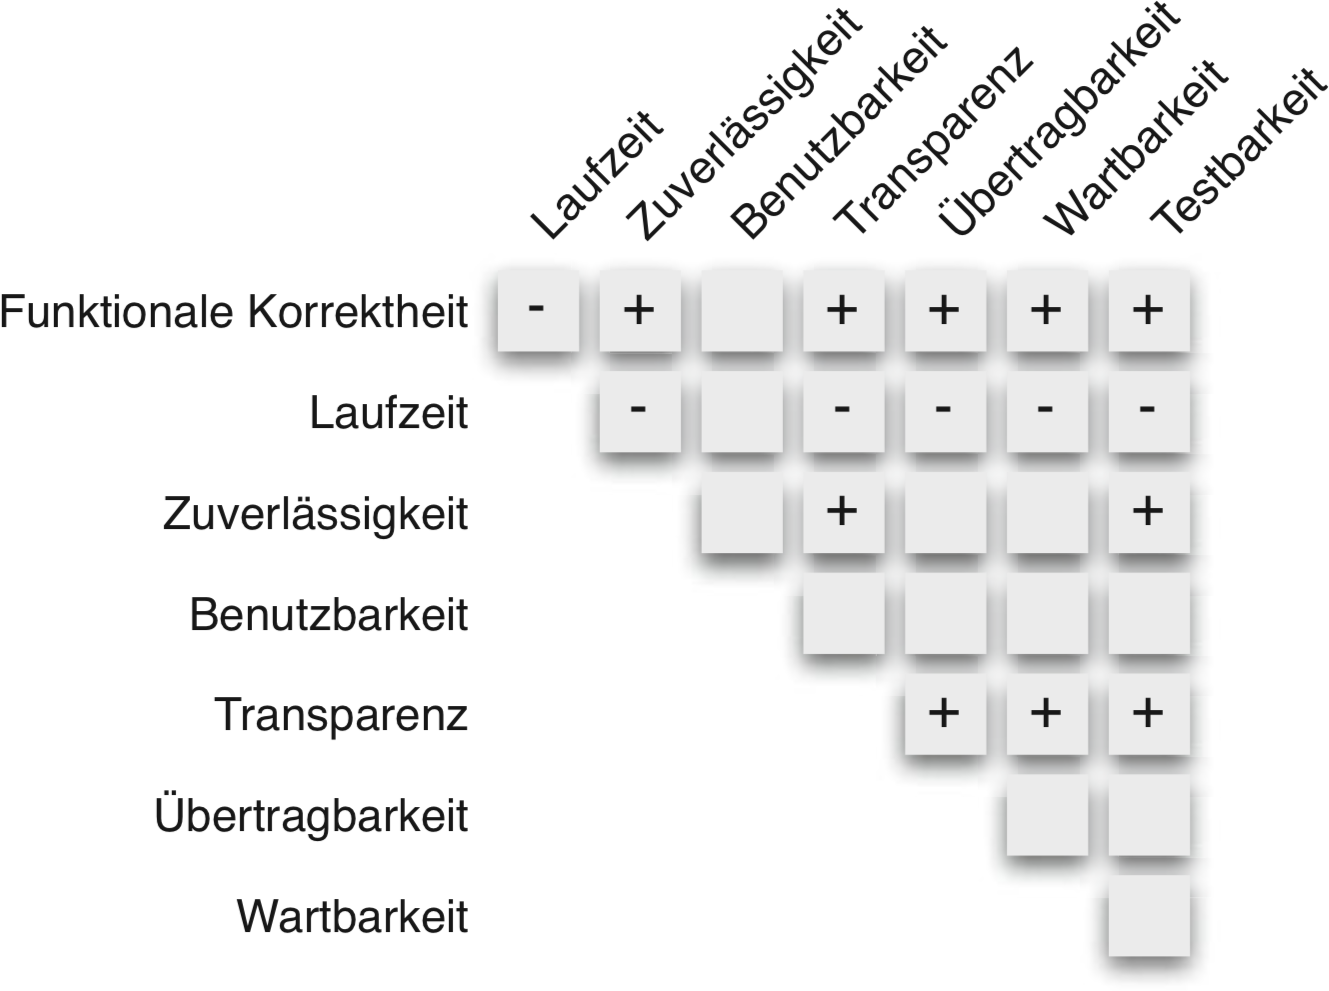
\includegraphics[width=0.6\textwidth]{img/korrelationsmatrix-kriterien.png}
    \caption[Korrelationsmatrix Qualitätskriterien]{Korrelationsmatrix Qualitätskriterien~\footcite[][S. 11, Abb. 1.3]{hoffmann_software_qualitat_2013}}\label{fig:Korrelationsmatrix Qualitätskriterien}
  \end{figure}
\end{savenotes}

\newpage
\section{Kennzahlen}

Software-Metriken helfen uns dabei, bestimmte (Qualitäts-) Merkmale beziehungsweise Kenngrößen eines Software-Systems systematisch und quantitativ zu erfassen.
Ziel ist es dabei, diese oft versteckten Merkmale sichtbar und vergleichbar zu machen.
Ein einfaches Beispiel ist die \ac{LOC}-Metrik, die die gesamte Anzahl an Zeilen Code darstellt und als grobes Maß für die Komplexität verwendet werden kann.

\begin{savenotes}
  \begin{figure}[H] 
    \centering
       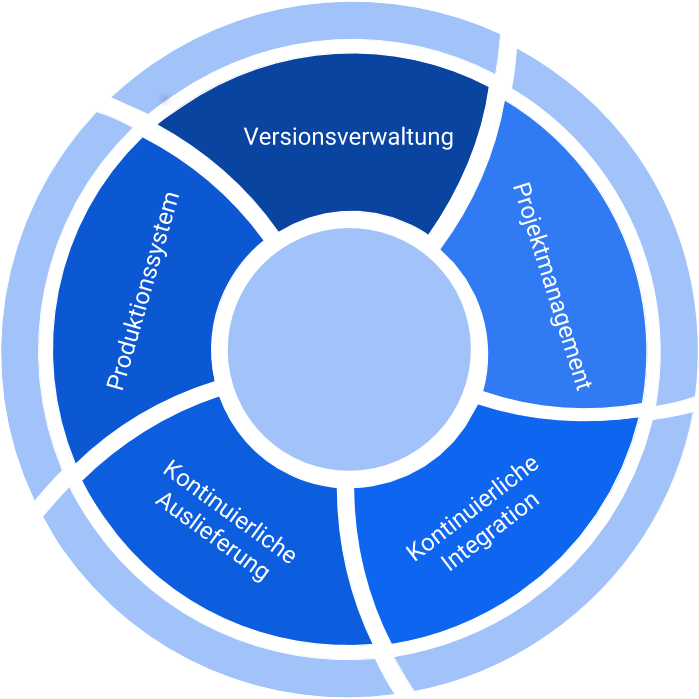
\includegraphics[width=0.6\textwidth]{img/software-development-lifecycle.png}
    \caption[Softwareentwicklungsprozess]{Softwareentwicklungsprozess~\label{fig:sdlc}}
  \end{figure}
\end{savenotes}

Im Entwicklungsprozess werden in den unterschiedlichen Systemen und Prozessschritten Daten erzeugt, die als Kennzahlen oder direkt als Metriken genutzt werden können.
Abbildung~\ref{fig:sdlc} zeigt die einzelnen Schritte und Systeme im Entwicklungsprozess.

\newpage
\subsection[Versionsverwaltung]{Versionsverwaltung~\footcite[vgl.][S.62ff]{davis_agile_2015}}

Das \ac{VCS} befindet sich nah an der Arbeit der Entwickler, da hier der Quellcode des Produkts verwaltet wird.
Daher können hier Daten darüber gesammelt werden, wie viel gearbeitet und auch wie viel zusammengearbeitet wird.
Um bestmögliche Daten zu bekommen, sollten verteilte Versionskontrollsysteme wie Git verwendet und mit Pull Requests gearbeitet werden.

\begin{description}
  \item[\ac{CLOC}] \hfill \\ Anzahl der geänderten Code Zeilen.
  \item[\ac{CLOC} pro Entwickler] \hfill \\ Anzahl der geänderten Zeilen im Quellcode pro Entwickler.
  \item[Commits] \hfill \\ Gesamtzahl an Commits in einem bestimmten Zeitraum.
  \begin{description}
    \item[Commits pro Entwickler] \hfill \\ Gesamtzahl an Commits in einem bestimmten Zeitraum pro Entwickler.
    \item[Kommentare pro Commit] \hfill \\ Anzahl der Kommentare pro Commit.
    \item[\ac{CLOC} pro Commit] \hfill \\ Anzahl der geänderten Zeilen im Quellcode pro Commit.
  \end{description}
  \item[Pull Requests] \hfill \\ Gesamtzahl an Pull Requests in einembestimmten Zeitraum.
  \begin{description}
    \item[Gemergte Pull Requests] \hfill \\ Anzahl erfolgreicher Pull Requests ineinem bestimmten Zeitraum.
    \item[Abgelehnte Pull Requests] \hfill \\ Anzahl abgelehnter Pull Requests in einem bestimmten Zeitraum.
    \item[Kommentare pro Pull Request] \hfill \\ Anzahl der Kommentare pro Pull Request.
  \end{description}
\end{description}

\newpage
\subsection[Projektmanagement]{Projektmanagement~\footcite[vgl.][S.37ff]{davis_agile_2015}}

In einem \ac{PTS} werden Aufgaben definiert und zugewiesen, Bugs verwaltet und Arbeitszeit mit Aufgaben verknüpft.
Hier können Daten über das Projektverständnis des Teams, die Geschwindigkeit und vor allem die Konsistenz der Arbeit gesammelt werden.
Um bestmögliche Daten erhalten zu können, gibt es folgende Empfehlungen:
\begin{itemize}[noitemsep]
  \item \ac{PTS} wird von allen genutzt
  \item Aufgaben mit möglichst vielen Tags versehen
  \begin{itemize}
    \item Aufgaben kategorisieren (nach ``gut'', ``ok'' und ``schlecht'')
  \end{itemize}
  \item Aufgaben schätzen
  \item gemeinsam eine \ac{DoD} festlegen
\end{itemize}
Jede Arbeit, die am \ac{PTS} vorbei geht, fällt später bei der Auswertung der Daten durch das Raster.
Durch das Taggen der Aufgaben können später Korrelationen ausgewertet werden, vor allem auch durch das Taggen, wie gut die Aufgabe abgelaufen ist.
Nur wenn die Aufgabe geschätzt ist, kann festgestellt werden, ob richtig geschätzt wurde oder wie viele Ausreißer es gibt. Dazu muss auch die Arbeitszeit auf der Aufgabe gespeichert werden.
Die \ac{DoD} hilft allgemein den Prozess zu verbessern und Rückläufe im Arbeitsablauf zu minimieren.

Dadurch ergeben sich folgende Kennzahlen aus einem \ac{PTS}:
\begin{description}
  \item[Burn Down] \hfill \\ Die Anzahl erledigte Arbeit über die Zeit. Liefert einen Richtwert, wo man sich gerade im Sprint befindet, verglichen zum Commitment.
  \item[Velocity] \hfill \\ Eine relative Messung der Konsistenz erledigter Arbeit über die Sprints.
  \item[Cummulative Flow] \hfill \\ Zeigt wie viel Aufgaben nach Status dem Team zugewiesen sind über die Zeit.
  \item[Lead Time] \hfill \\ Zeit zwischen Start und Abschluss einer Aufgabe, vor allem interessant bei Kanban.
  \item[Bug Counts] \hfill \\ Die Anzahl an Bugs über die Zeit.
  \begin{description}
    \item[Bug-Erzeugungsrate] \hfill \\ Anzahl Bugs nach Erstellungsdatum.
    \item[Bug-Fertigstellungsrate] \hfill \\ Anzahl Bugs nach Erledigungsdatum.
  \end{description}
  \item[Aufgaben-Volumen] \hfill \\ Die Anzahl der Aufgaben und kann der Schätzung gegenübergestellt werden, um die Größe der Aufgaben oder ungeplante Arbeit aufzuzeigen.
  \item[Aufgaben-Rückfälligkeit] \hfill \\ Zeigt auf, wie oft Aufgaben im Arbeitsablauf rückwärts gehen.
\end{description}

\subsection[Kontinuierliche Integration und Auslieferung]{Kontinuierliche Integration und Auslieferung~\footcite[vgl.][S.84ff]{davis_agile_2015}}

\ac{CI}- und \ac{CD}-Systeme stellen sicher, dass die erstellte Software zu jedem Zeitpunkt auslieferbar ist, in dem sie zu definierten Zeitpunkten automatisch neu gebaut und ausgeliefert wird.
In einer solchen Build-Pipeline können sehr viel nützliche Daten erzeugt werden, vor allem mit Tools für statische Analysen (wie zum Beispiel SonarQube~\footcite[][]{sonarqube}).
Diese Systeme sind aber auch jene Elemente im Softwareentwicklungsprozess, die von Team zu Team am meisten variieren können.
Daher hängen die erzeugten Daten auch stark vom jeweiligen Setup ab.
Grundsätzlich können aber folgende Kennzahlen aus diesen Systemen ermittelt werden:

\begin{description}
  \item[Build-Dauer] \hfill \\ Geschätzte und tatsächliche Dauer der Builds.
  \item[Build-Status] \hfill \\ Es können die Anzahl der erfolgreichen und fehlerhaften Builds gegenüber gestellt werden.
  \item[Build-Frequenz] \hfill \\ Wie oft wird ein Build ausgelöst.
  \item[Test Reports] \hfill \\ Anzahl erfolgreicher und fehlerhafter Tests, Gesamtdauer der Tests.
  \item[Code Coverage] \hfill \\ Wie viel Prozent des Quellcodes ist mit Tests abgedeckt.
  \item[Stresstests oder Benchmarking] \hfill \\ Wird oft im Build Prozess mit getestet mit Tools wie JMeter~\footcite[][]{jmeter} oder Gatling~\footcite[][]{gatling}.
\end{description}

\newpage
\subsection[Produktionssystem]{Produktionssystem~\footcite[vgl.][S.107ff]{davis_agile_2015}}

Daten aus den Produktionssystemen können gesammelte \ac{APM}- oder auch \ac{BI}-Kennzahlen sein.
Diese Kennzahlen ermöglichen Aussagen, ob die Kunden zufrieden sind und wie das System arbeitet.
Die \ac{BI}-Kennzahlen sollten möglichst nahe am Entwicklungsteam gehalten werden, damit es verstehen kann, wie die Kunden die Applikation nutzen.
Dazu können Frameworks wie StatsD~\footcite[][]{statsd} und Atlas~\footcite[][]{atlas} verwendet werden.
Im Produktionssystem können folgende Kennzahlen ermittelt werden:

\begin{description}
  \item[CPU Nutzung] \hfill \\ Auslastung der Prozessoren über die Zeit.
  \item[Heap Size] \hfill \\ Auslastung des Heap über die Zeit.
  \item[Fehlerraten] \hfill \\ Anzahl Fehler über die Zeit (kann aus dem Logging kommen).
  \item[Antwortzeiten] \hfill \\ Dauer der Verarbeitung bestimmter Anfragen.
  \item[Benutzeranzahl] \hfill \\ Anzahl gleichzeitiger Benutzer in der Applikation über die Zeit.
  \item[Aufenthaltsdauer] \hfill \\ Verweildauer der Benutzer auf bestimmten Seiten.
  \item[Conversion Rate] \hfill \\ Anzahl Benutzer die zu Kunden wurden.
  \item[Semantisches Logging] \hfill \\ Ermöglicht es, beim Logging strukturierte Daten auszugeben, zum Beispiel: was suchen Benutzer auf bestimmten Seiten.
  \item[Verfügbarkeit] \hfill \\ Verfügbarkeit der Applikation über die Zeit.
\end{description}

\subsection{Übersicht Kennzahlen im Entwicklungsprozess}

Die Metriken finden sich nochmal als Tabelle dargestellt und mit den dazugehötigen Fragen, die sie jeweils beantworten, im Anhang~\ref{appendix:metrics}.

\newpage
\section{Metriken}

Eine Softwaremetrik wird vom \ac{IEEE} Standard 1061 von 1998 folgendermaßen definiert:
\begin{quote}
  ``Eine Softwarequalitätsmetrik ist eine Funktion, die eine Software-Einheit in einen Zahlenwert abbildet, welcher als Erfüllungsgrad einer Qualitätseigenschaft der Software-Einheit interpretierbar ist.''\footcite[vgl.][S.3]{ieee-1061}
\end{quote}

Vereinfacht gesagt, ist eine Metrik eine oder mehrere Kennzahlen, die mithilfe einer Funktion ein Qualitätsmerkmal in einen Zahlenwert abbilden.
Eine Kennzahl kann daher auch schon direkt eine Metrik sein, wenn sie in der Lage ist, ein gewünschtes Qualitätsmerkmal abzubilden.

\subsection[Veröffentlichung von Metriken]{Veröffentlichung von Metriken~\footcite[vgl.][S.177ff]{davis_agile_2015}}

Metriken können auf verschiedene Art und Weise veröffentlicht werden. Zwei mögliche Beispiele sind Dashboards oder Emails.
Grundsätzlich sollte beachtet werden, dass man sich bei der Veröffentlichung von Metriken innerhalb der Grenzen und Gewohnheiten des Unternehmens bewegen sollte.
Außerdem sollte auf folgende Punkte geachtet werden:

\begin{description}
  \item[Dashboards] \hfill
  \begin{itemize}[noitemsep]
    \item den Zugriff innerhalb der Firma nicht einschränken
    \begin{itemize}[noitemsep]
      \item aber als intern ansehen
    \end{itemize}
    \item muss nach den Bedürfnissen der Teams anpassbar sein
    \item Metriken werden als Werkzeug gesehen, nicht als Waffe (gegen andere Teams oder Personen)
    \item Page Tracking verwenden, um das Nutzungsverhalten zu verstehen
  \end{itemize}
  \item[Emails] \hfill
  \begin{itemize}[noitemsep]
    \item aus dem Dashboard optional machen (sonst landen sie schnell automatisch im Spam-Ordner)
    \item minimal erforderliche Daten, den Rest verlinken zum Dashboard
    \item den Richtigen Rhytmus finden (zwischen oft genug informieren und nerven)
  \end{itemize}
\end{description}

Arbeitet ein Unternehmen beispielsweise viel mit Reports via Email, dann kann ein reines Dashboard weniger Anerkennung finden. Hier könnte beispielsweise eine Übersicht per Mail versendet und mit Links zum Dashboard versehen werden.

\subsection{Allgemeine Metriken}

Es gibt einige allgemeine Metriken, die für jedes Scrum Team von Bedeutung sind.
Wie stark, kann jedes Team selbst entscheiden, aber sie sollten nicht aus den Augen verloren werden.

\begin{itemize}
  \item Metrik 1
\end{itemize}

\subsection[Eigene Metriken erstellen]{Eigene Metriken erstellen~\footcite[vgl.][S.127ff]{davis_agile_2015}}

Um eigene Metriken erstellen zu können sind 2 Dinge notwendig:
\begin{itemize}
  \item Daten
  \item eine Funktion, um die Metrik zu berechnen
\end{itemize}

Dabei sollte darauf geachtet werden,
\begin{itemize}
  \item dass man auf die Metrik reagieren kann (Dinge, die einen stören und die man nicht ändern kann, frustrieren oder demotivieren)
  \item dass sich die Metrik nach den Team-Grundsätzen und Kerngeschäften ausrichtet
  \item dass die Metrik für sich alleine stehen kann
\end{itemize}

\subsection[Agile Prinzipien messen]{Agile Prinzipien messen~\footcite[vgl.][S.201ff]{davis_agile_2015}}

Um die agilen Prinzipien messen zu können, muss zuerst herausgefunden werden, was die Kernaussagen dieser Prinzipien sind.
Dies kann zum Beispiel grafisch, durch die Erstellung einer Wortwolke, wie in Abbildung~\ref{fig:wordcloud_principles} ersichtlich, erreicht werden.

\begin{savenotes}
  \begin{figure}[H] 
    \centering
    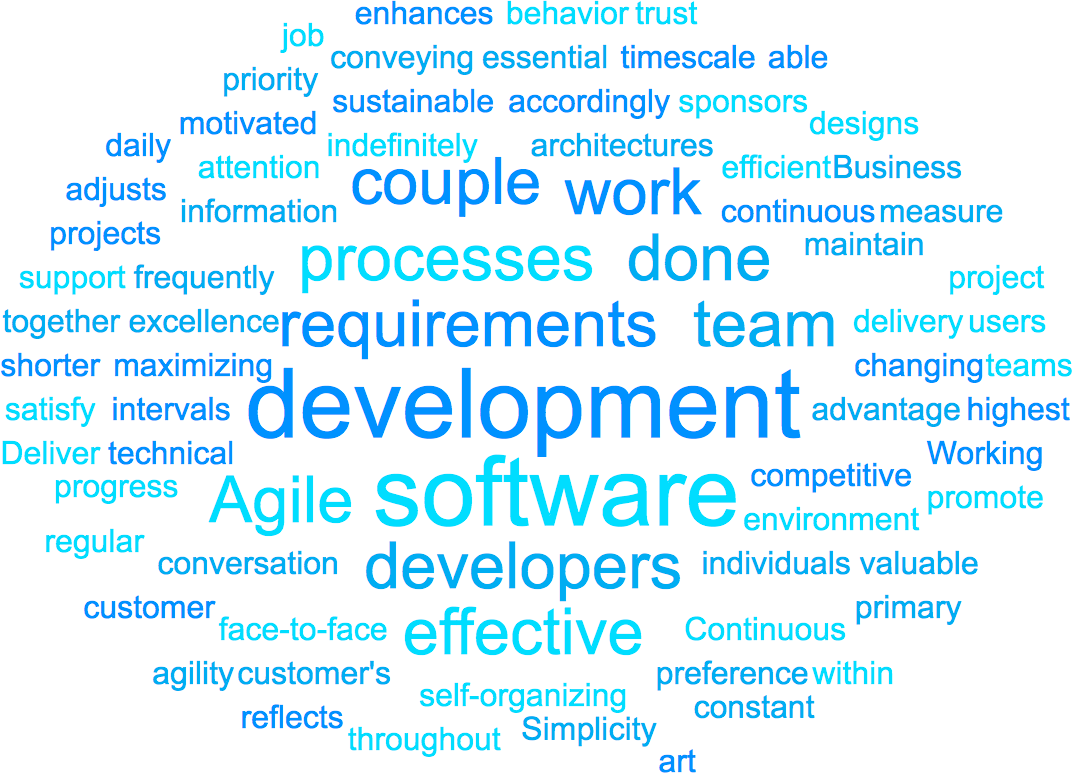
\includegraphics[width=0.9\textwidth]{img/principles-wordcloud.png}
    \caption{Agile Prinzipien als Wortwolke}\label{fig:wordcloud_principles}
  \end{figure}
\end{savenotes}

Aus dieser Wortwolke heben sich neben den Begriffen ``development'' und ``software'' vor allem auch die Begriffe ``team'', ``processes'', ``effective'' und ``requirements'' hervor.
Mithilfe dieser Begriffe lassen sich folgende vier Punkte ableiten:

\begin{itemize}[noitemsep]
  \item Effektive Software
  \item Effektiver Prozess
  \item Effektives Team 
  \item Effektive Anforderungen 
\end{itemize}

Für jeden dieser vier Punkte sind Metriken aus den unterschiedlichsten Systemen anwendbar~\footcite[vgl.][S.219ff]{davis_agile_2015}:

\begin{description}
  \item[Effektive Software] \hfill
  \begin{itemize}[noitemsep]
    \item erfolgreiche / fehlerhafte Builds
    \item Business-Metriken
    \item Status der Applikation
    \begin{itemize}[noitemsep]
      \item Fehlerraten
      \item CPU/Speicher Auslastung
      \item Antwort- / Transaktionszeiten
      \item Heapgröße / Garbage Collection / Anzahl Threads
    \end{itemize}
  \end{itemize}
  \item[Effektiver Prozess] \hfill
  \begin{itemize}[noitemsep]
    \item Velocity
    \item \ac{PTS} und \ac{VCS} Kommentare
    \item erfolgeiche Releases
  \end{itemize}
  \item[Effektives Team] \hfill
  \begin{itemize}[noitemsep]
    \item Lead Time
    \item \ac{MTTR}
    \item Deploy-Frequenz
    \item fehlerhafte Builds
  \end{itemize}
  \item[Effektive Anforderungen] \hfill
  \begin{itemize}[noitemsep]
    \item Rückläufigkeit
    \item Lead Time
    \item \ac{MTTR}
    \item Velocity
  \end{itemize}
\end{description}

\chapter{Zielsetzung}

\section{Vorgehensmodell}

Entwicklung eines Vorgehensmodells zur Bestimmung von relevanten Qualitätsmetriken von Teams.

\section{Software}

Entwicklung einer Software zur Darstellung von Qualitätsmetriken von Teams.

\chapter{Methodik}

\section{Vorgehensmodell}

\subsection{\ac{GQM}}

Befragung Team blabla

\subsubsection{Vorauswahl}

Um eine Vorauswahl an Metriken treffen zu können, wurden alle bisherigen Retrospektiven (es waren genau 15) analysiert und eine Topliste von Schlagwörtern der folgenden Fragestellungen aus den Retrospektiven erstellt:
\begin{enumerate}
    \item Welche guten Entscheidungen haben wir getroffen?
    \item Was haben wir gelernt?
    \item Was können wir besser machen?
    \item Was nervt uns noch immer?
\end{enumerate}

Dazu wurden die Ergebnisse in eine ElasticSearch Datenbank gespeichert und über eine sogenannte Terms Aggregation die wichtigsten Schlagwörter analysiert.
Bei der Indizierung werden die Wörter normalisiert, deshalb die teilweise andere Schreibweise (zum Beispiel wird aus Issue der Term issu).
\newline
Aus den Ergebnissen in Anhang~\ref{appendix:retros} ist ersichtlich, dass

\section{Software}

Technologien, Plattform, etc.

\subsection{Architektur}

Abbildung~\ref{fig:position_architecture} zeigt die Position und Abbildung~\ref{fig:overview_architecture} die grobe Architektur der Software (Agile Metrics).
Die Software bildet eine Schnittstelle zwischen den einzelnen Systemen des Entwicklungsprozesses und dem System zur Darstellung der Metriken (in diesem Fall ElasticSearch und Kibana).

\begin{savenotes}
    \begin{figure}[H] 
        \centering
            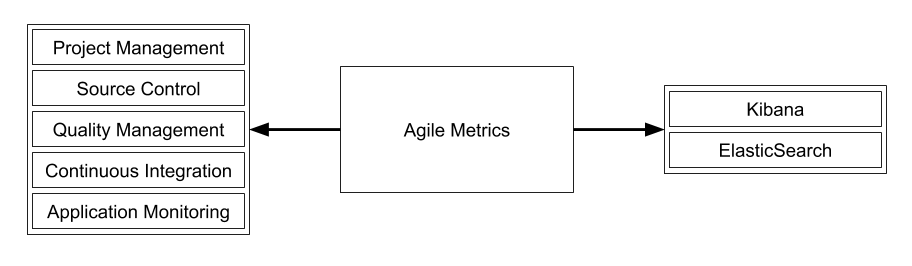
\includegraphics[width=0.8\textwidth]{img/position-overview.png}
        \caption{Position der Software}\label{fig:position_architecture}
    \end{figure}
\end{savenotes}

\begin{savenotes}
    \begin{figure}[H] 
        \centering
            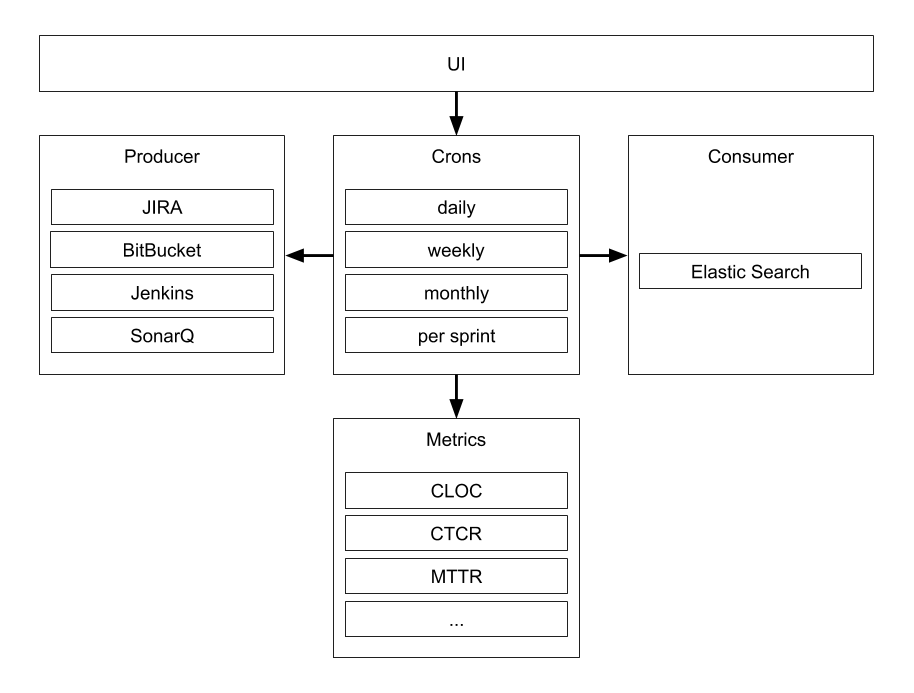
\includegraphics[width=0.8\textwidth]{img/architecture-overview.png}
        \caption{Übersicht der Software-Architektur}\label{fig:overview_architecture}
    \end{figure}
\end{savenotes}

\begin{description}
    \item[UI] \hfill \\ Bietet eine grafische Benutzeroberfläche zur Konfiguration.
    \item[Producer] \hfill \\ Sind Schnittstellen zu allen Systemen, die Messdaten erzeugen.
    \item[Crons] \hfill \\ Zeitsteuerung der Messdaten-Abfrage (z.B. täglich oder pro Sprint).
    \item[Metrics] \hfill \\ Hier können aus Messdaten direkt Metriken erstellt werden.
    \item[Consumer] \hfill \\ Sind Schnittstellen zu allen Systemen, die Messdaten und Metriken konsumieren.
\end{description}

\chapter{Ergebnisse}

\section{Vorgehensmodell}

\ldots Ergebnis der Ausarbeitung.

\section{Einführung des Vorgehensmodells}

\ldots bei Gebrüder Weiss.

\section{Inbetriebnahme der Software}

\ldots allgemein, Beschreibung der Connectoren, Darstellungsarten, etc.

\subsection{Visualisierte Ergebnisse}

\begin{savenotes}
    \begin{figure}[H] 
        \centering
            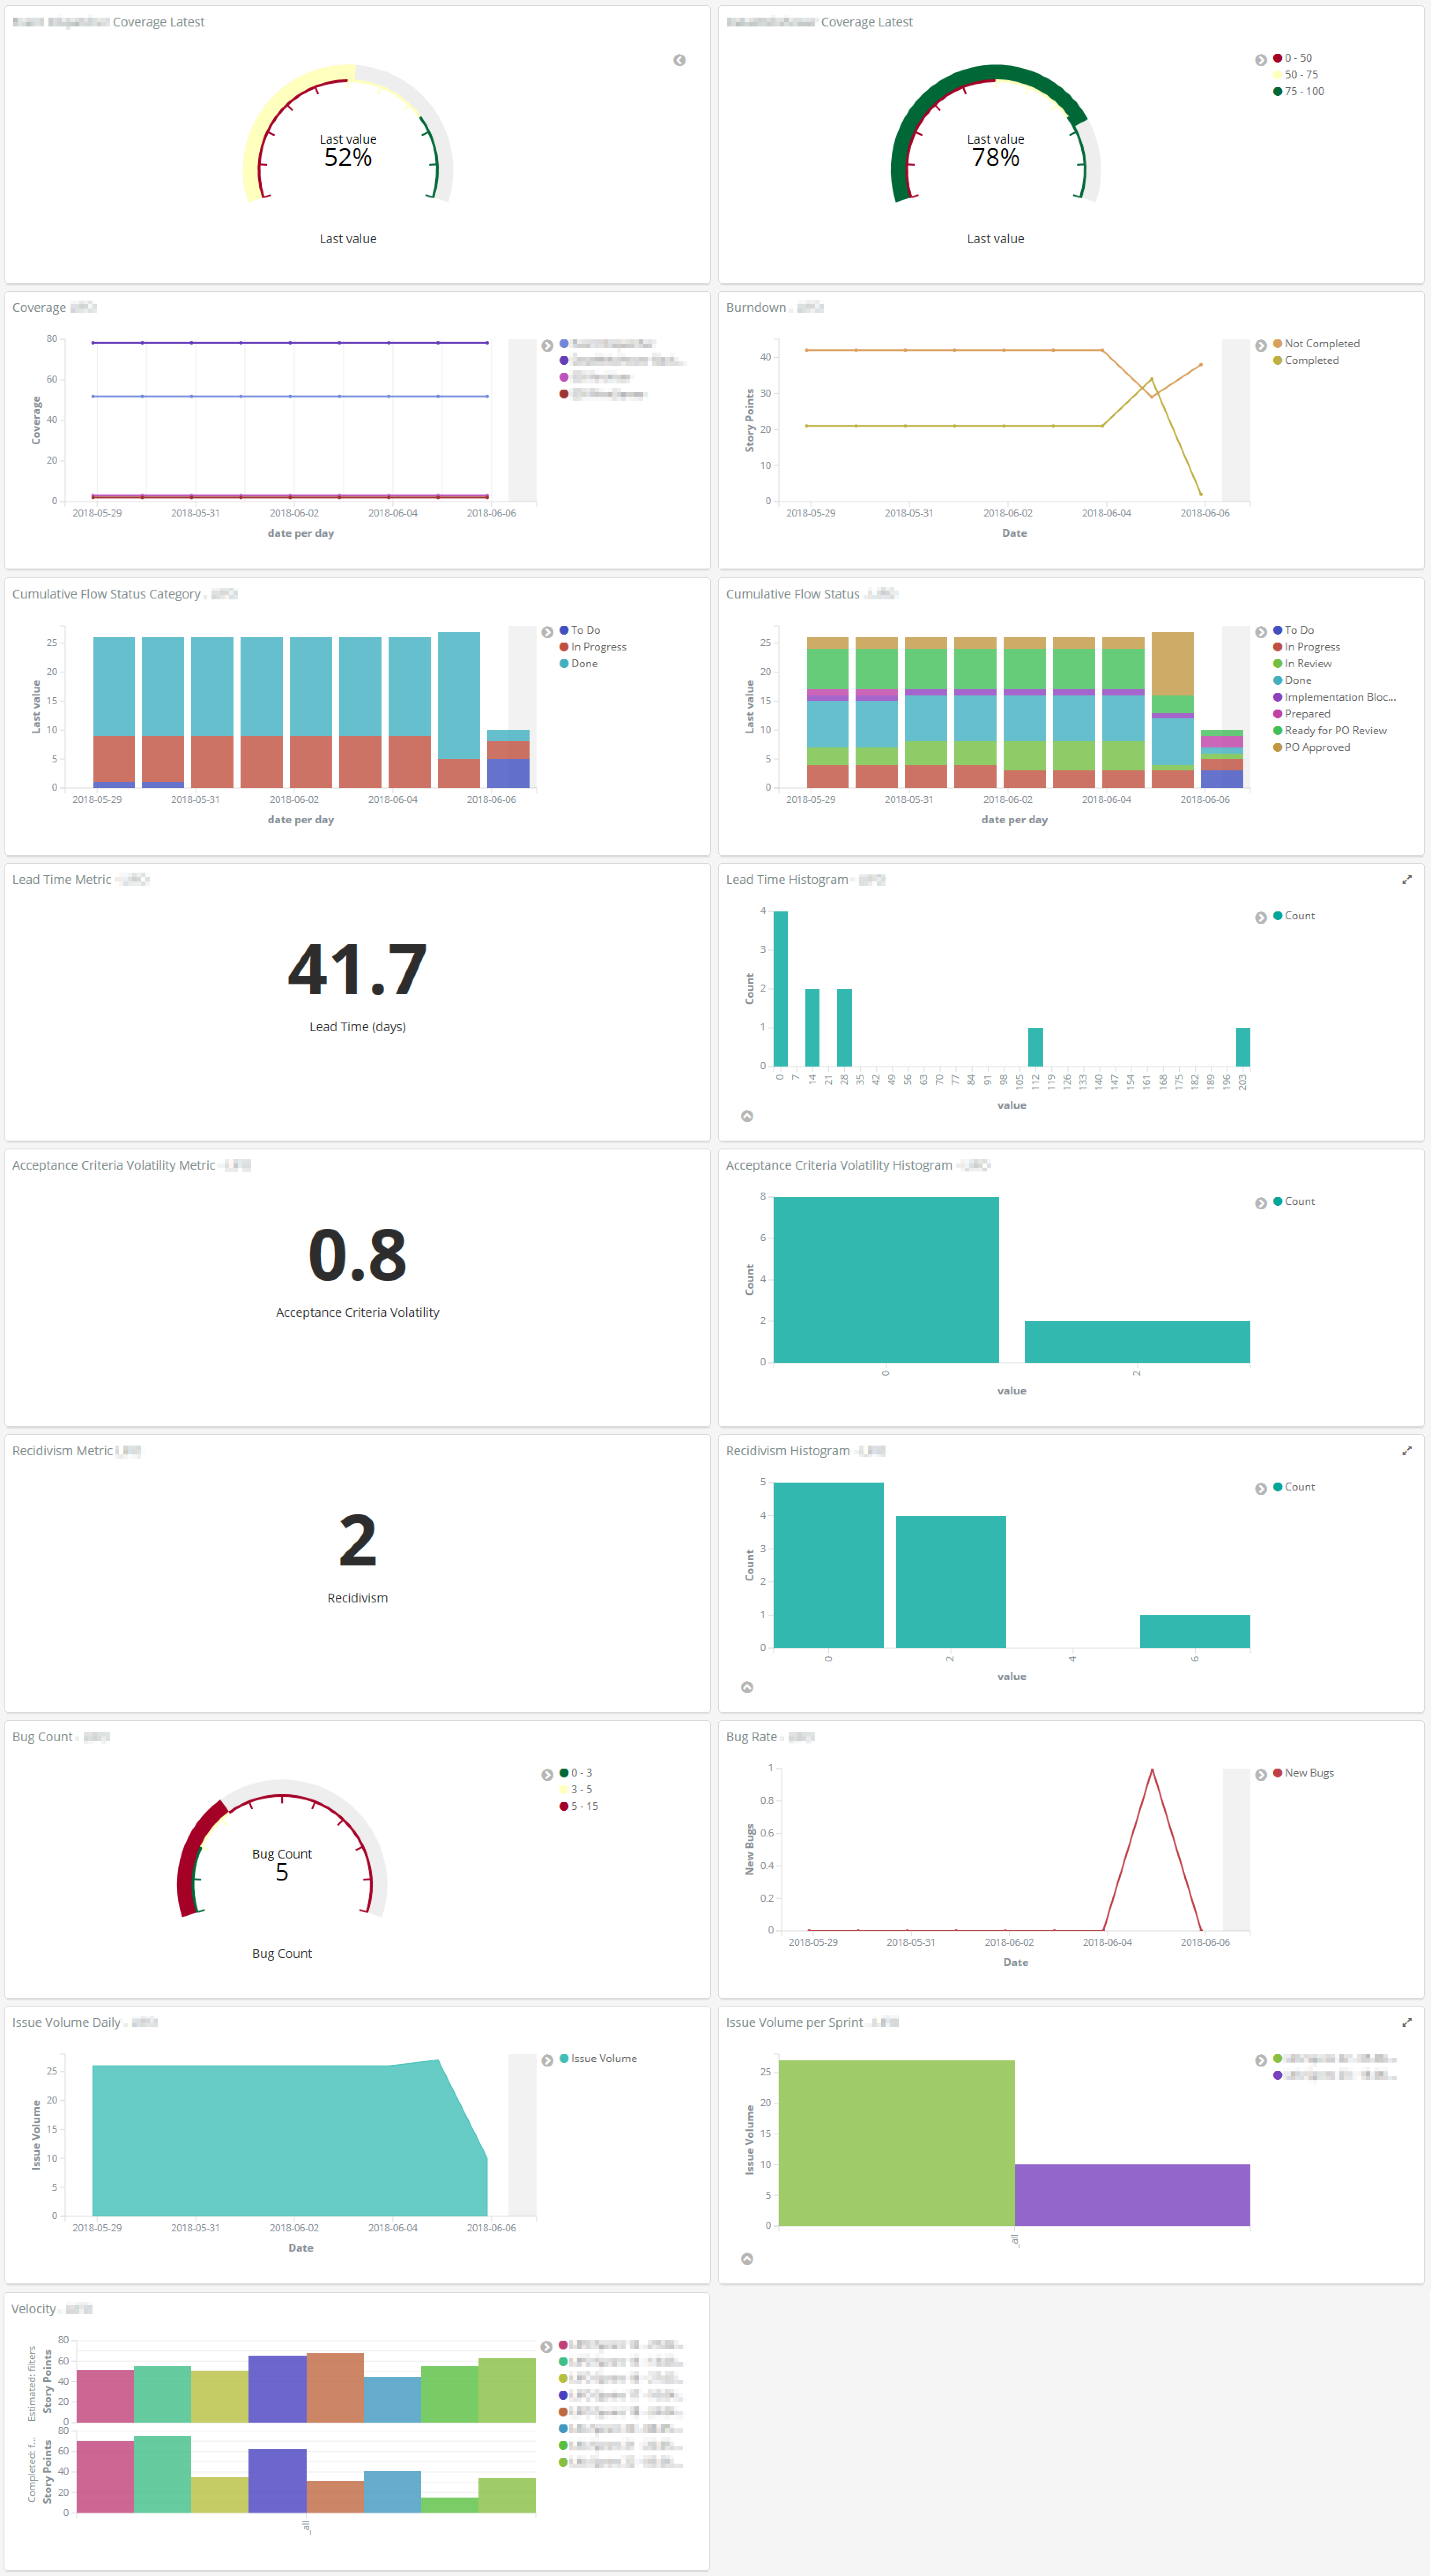
\includegraphics[width=1.0\textwidth]{img/dashboard.png}
        \caption{Dashboard mit den Metriken}\label{fig:dashboard}
    \end{figure}
\end{savenotes}

\section{Evaluierung des Vorgehensmodells}

\ldots wie wurde es angenommen? Welche Auswirkungen hatte es?

\chapter{Schlussfolgerungen}

In dieser Arbeit konnte gezeigt werden, dass mithilfe des \ac{GQM}-Modells, ergänzt durch eine Umfrage im entsprechenden Scrum Team, Metriken ermittelt werden können, die es ermöglichen, die Schwachstellen in einem Produkt und im agilen Prozess in Zahlen zu fassen.
Diese Metriken ermöglichen es dem agilen Team, seine Fortschritte bei den Retrospektiven nachvollziehbar bewerten und weitere Maßnahmen treffen zu können.
Außerdem können durch die Kombination unterschiedlicher Metriken Korrelationen zwischen bestimmten Metriken nachgewiesen oder widerlegt werden.
Reichen die bekannten Metriken in der Literatur nicht aus, können auch eigene erstellt werden.
\\
Die entwickelte Software hilft dabei, die Daten aus den unterschiedlichen Systemen im Entwicklungsprozess als Metriken aufzubereiten und zu speichern.
Dabei wurde bei der Architektur auf Fehlertoleranz und einfache Erweiterbarkeit geachtet, sodass ein einfacher Betrieb und eine Erweiterung der unterstützten Systeme und Metriken möglich ist.
Für einen einfachen Zugang und eine uneingeschränkte Erweiterbarkeit wurde der Quellcode der Software unter der quelloffenen MIT-Lizenz veröffentlicht.
Bei der Visualisierung von Metriken bietet Kibana eine geeignete Plattform, um aus den gespeicherten Metriken einfach Dashboards mit unterschiedlichen Visualisierungen bereitzustellen.
Dabei muss berücksichtigt werden, dass Entwicklerinnen, Scrum Master und Product Owner jeweils unterschiedliche Interessen an den Metriken haben.
Durch eine geeignete Gruppierung der Metriken können den unterschiedlichen Teammitgliedern auf einen Blick die wichtigsten Metriken dargestellt werden.
Dadurch wird das Dashboard auch regelmäßig genutzt und somit die Akzeptanz noch weiter erhöht.
Der Einsatz der Software ermöglicht den Aufbau einer zentralen Stelle, an der die Metriken aus allen relevanten System gesammelt, dargestellt und kombiniert werden können.
\\
Schwachstellen wurden bei der Art der Darstellung mancher Metriken identifiziert.
Hier war der Wunsch nach einer besseren Beschreibung der Metriken, um Diskussionen über deren Bedeutung zu vermeiden.
Zusätzlich soll eine Beschreibung von Zielen helfen, die Absicht hinter Metriken beschreiben zu können.
Bei manchen Darstellungen wurden noch zusätzliche Detailinformationen zu den einzelnen Datensätzen gewünscht, um Ausreißer leichter identifizieren zu können.
Trotzdem wurde das erstellte Dashboard trotz des relativ kurzen Testzeitraums von nicht ganz drei Sprints gut angenommen.
Bei der Evaluierung wurde auch klar, dass die Teammitglieder bereits erkannten, wie sie das Dashboard persönlich am besten nutzen.
\\
Durch den Einsatz der entwickelten Software und der vorgestellten Modelle zur Identifizierung von relevanten Metriken, kann die Qualität in einem agilen Team dadurch erhöht werden, dass Qualitätsprobleme durch Metriken sichtbar gemacht und in den Retrospektiven Gegenmaßnahmen dafür getroffen werden können.

\chapter{Zusammenfassung}

Scrum ist inzwischen eine sehr weit verbreitete agile Vorgehensweise von Entwicklungsteams.
Dabei ist die Reflexion der bisherigen Arbeit eine der Grundideen von Scrum, der sogenannte Empirismus.
Empirismus ist die Theorie, dass Wissen aus Erfahrung erlangt wird.
Um auf Basis dieses Wissens Entscheidungen zu treffen, benötigt ein Scrum-Team Kennzahlen.
Solche Kennzahlen können in Form von Metriken in einem leicht zugänglichen Dashboard visualisiert werden.
Metriken dienen hauptsächlich dazu, Qualitätsmerkmale eines Produkts oder Prozesses als Zahlenwert darzustellen.
\\
Eingeführt wurde ein solches Dashboard bei einem relativ fortgeschrittenen Scrum-Team in einem Unternehmen mit rund 6700 Mitarbeitern.
Gestartet wurde mit der Ermittlung von geeigneten Metriken für das Team.
Dazu wurden zuerst alle bisherigen Retrospektiven ausgewertet und basierend auf diesen Daten mit der \ac{GQM}-Methodik Metriken ermittelt.
Zusätzlich wurde aufgrund des erfahrenen Teams noch eine Umfrage gemacht, bei der den Teammitgliedern die gängigsten Metriken vorgestellt und in einer Skala von eins bis zehn nach Wichtigkeit bewertet wurden.
\\
Um diese ermittelten Metriken dann darzustellen, wurde eine leicht erweiterbare, quelloffene Software in Java erstellt, die alle relevanten Daten aus den Systemen im Entwicklungsprozess über Schnittstellen sammelt, aufbereitet und als Metriken in einer Datenbank speichert.
Konkret wurde der sogenannte Elastic Stack eingesetzt, also eine ElasticSearch Datenbank zur Speicherung und Kibana zur Visualisierung der Metriken und Bereitstellung über Dashboards.
Diese Metriken wurden anschließend vom Scrum-Team über den Zeitraum von nicht ganz drei Sprints getestet.
Dabei konnte gezeigt werden, dass je nach Rolle im Team zwar andere Metriken wichtig sind, aber jeder das Dashboard für sich zu nutzen wusste.
Besonders der Scrum-Master bekam schnell einen Eindruck, welche Möglichkeiten dem Team dadurch eröffnet werden.

\section*{Ausblick}

Folgende Erweiterungen dieser Arbeit wären möglich:

\begin{description}
    \item[Testzeitraum] \hfill \\ Die Entwicklung des Teams und des Dashboards mit den Metriken könnte noch über einen längeren Zeitraum verfolgt werden, um ausführlichere Rückschlüsse über die Effektivität und den Nutzen zu ziehen.
    \item[Testumfang] \hfill \\ Der Testumfang kann auf mehrere Teams erweitert werden, um ein noch umfangreicheres Feedback zu bekommen.
    \item[Systeme] \hfill \\ Mehr unterstützte Systeme kann die Akzeptanz der Software erhöhen.
    \item[Metriken] \hfill \\ Auch neue Metriken erhöhen die Akzeptanz der Software und erlauben es Teams, noch mehr Einsicht in ihre Prozesse und Systeme zu erlangen.
    \item[Geschäftsebenen] \hfill \\ Das Dashboard könnte noch weiteren Ebenen im Unternehmen bereitgestellt werden, zum Beispiel dem Management, um eine Übersicht über den Gesamtprozess zu erlangen.
\end{description}


% Literaturverzeichnis:
\clearpage
\phantomsection{}
\addcontentsline{toc}{chapter}{Literaturverzeichnis}
\printbibliography{}

\chapter*{[evtl. Anhang]}  % evtl. ersetzen mit \chapter*{Anhang}
\addcontentsline{toc}{chapter}{[evtl. Anhang]}   % evtl. ersetzen mit \addcontentsline{toc}{chapter}{Anhang}
Formatvorlage für den Fließtext.

\chapter*{Eidesstattliche Erklärung}
\addcontentsline{toc}{chapter}{Eidesstattliche Erklärung}
Ich erkläre hiermit an Eides statt, dass ich die vorliegende Masterarbeit selbstständig und ohne Benutzung anderer als der angegebenen Hilfsmittel angefertigt habe. Die aus fremden Quellen direkt oder indirekt übernommenen Stellen sind als solche kenntlich gemacht. Die Arbeit wurde bisher weder in gleicher noch in ähnlicher Form einer anderen Prüfungsbehörde vorgelegt und auch noch nicht veröffentlicht.

\vspace{3cm}
\noindent
Dornbirn, am [Tag. Monat Jahr anführen]\hfill [Vor- und Nachname Verfasser/in]


\end{document}
